\documentclass{utfpr-pg}

\usepackage{cmap}
\usepackage[T1]{fontenc}
\usepackage{graphicx}
\usepackage{latexsym}
\usepackage{amssymb}
\usepackage{lipsum}
\usepackage{pdfpages}
\usepackage{float}
\usepackage{color,soul}
\usepackage{xcolor}
\usepackage{adjustbox}
\usepackage{quoting}
\usepackage{tocloft}
\usepackage[font=small,labelfont=bf]{caption}



\cftsetindents{section}{0em}{1.2cm}
\cftsetindents{subsection}{0em}{0.85cm}
\cftsetindents{subsubsection}{0cm}{0.65cm}
\cftsetindents{chapter}{0pt}{1.7cm}

\makeatletter

\renewcommand*\l@chapter{\@dottedtocline{0}{0em}{1.5cm}}
\makeatother

\graphicspath{{Imagens/}}

\DeclareFloatingEnvironment[
fileext=lod,
listname=Lista de Definições,
name=Definição,
placement=tbhp,
]{definicao}


\curso{}
\autor{ Alana Mafra Netto  \\  Everton Henrique Carneiro }
\titulo{Aplicativo para ensino de lógica de programação utilizando visão computacional}
\local{Curitiba}
\data{2020}
\preambulo{Monografia apresentada como requisito parcial de aprovação da disciplina de Trabalho de Conclusão de Curso de Engenharia da Computação da Universidade.\break}

\orientador{Dra Veronica Isabela Quandt}

% informações do PDF
\makeatletter
\hypersetup{
        % pagebackref=true,
        pdftitle={\@title},
        pdfauthor={\@author},
        pdfsubject={\imprimirpreambulo},
        pdfcreator={LaTeX with abnTeX2},
        colorlinks=false,
}
\makeatother

% Controle do espaçamento entre um parágrafo e outro:
\setlength{\parskip}{0.1cm}  % tente também \onelineskip

\makeindex
\begin{document}
% Retira espaço extra obsoleto entre as frases.
\frenchspacing

\imprimircapa
\imprimirfolhaderosto

% % Termo de aprovação
% 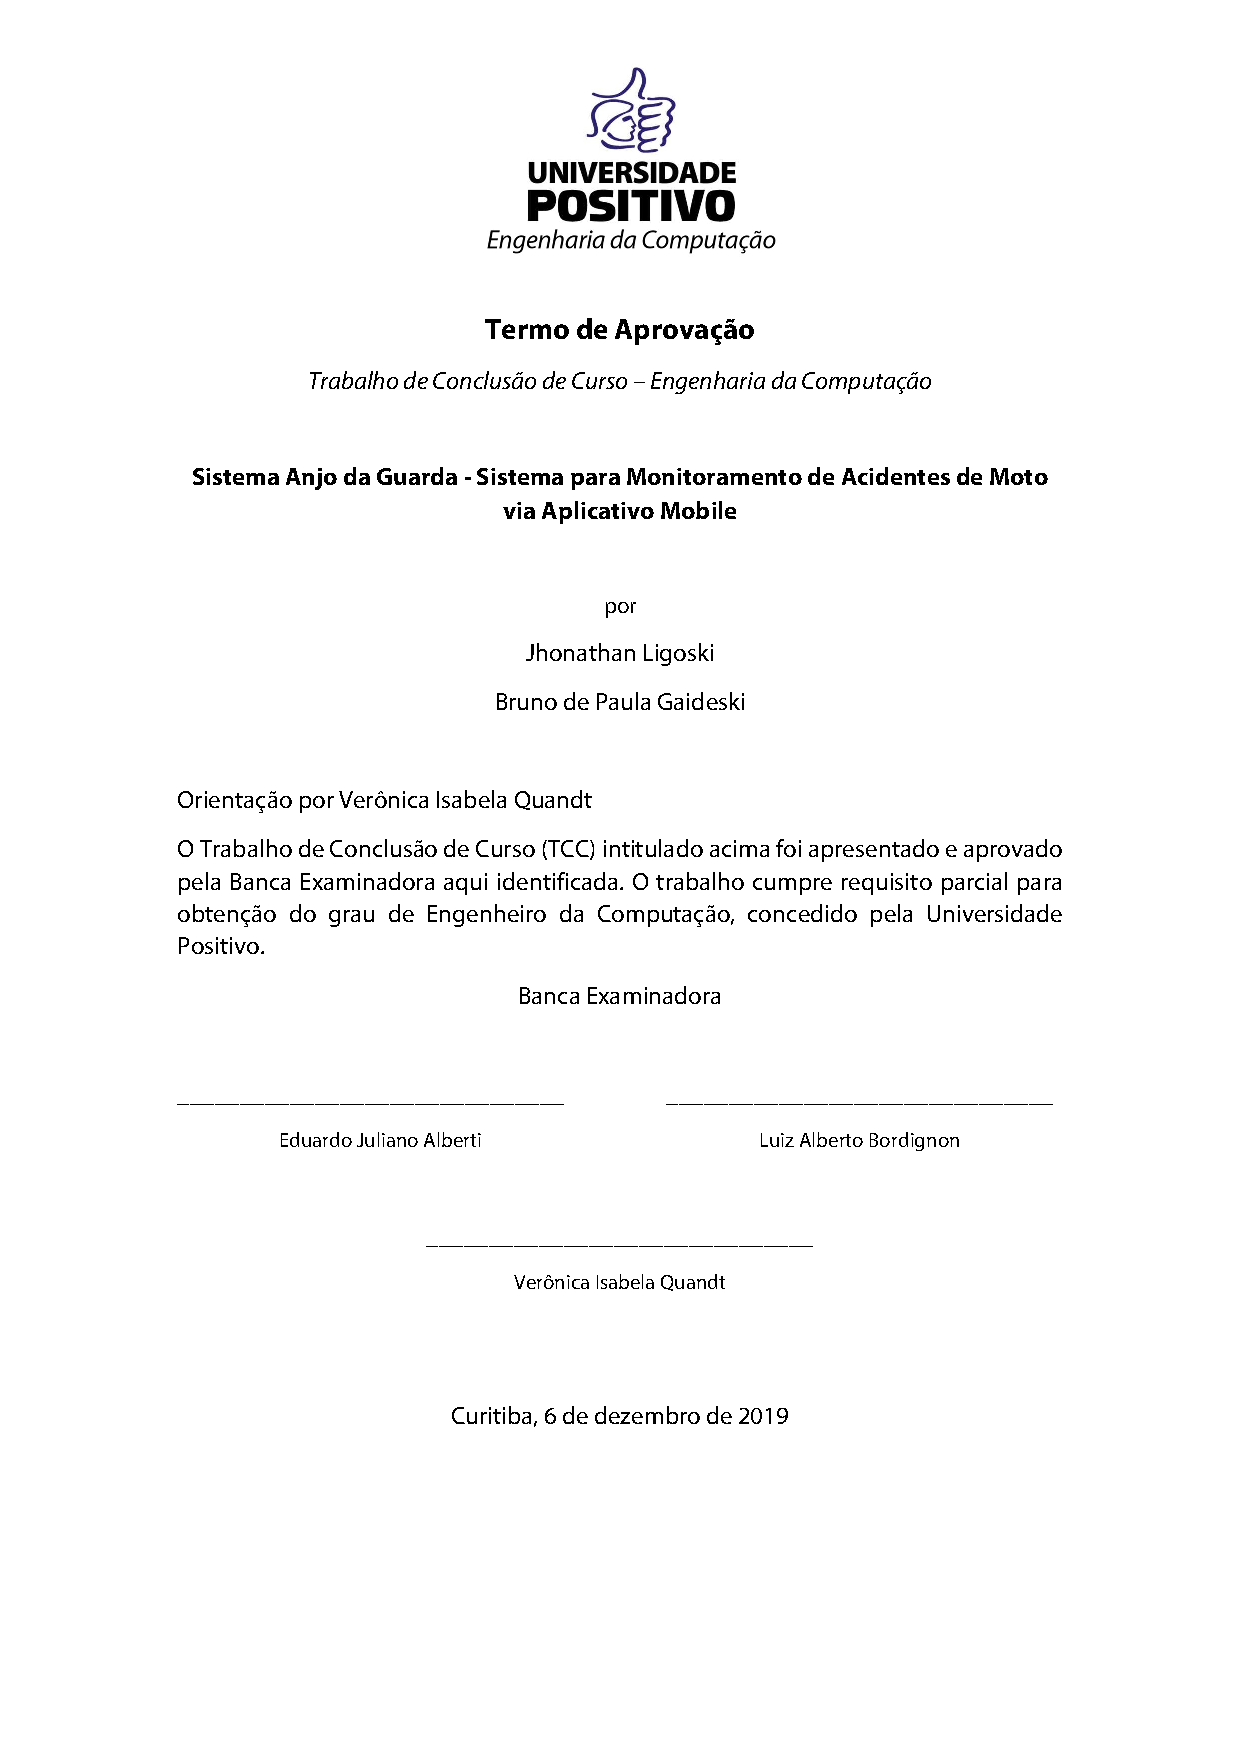
\includepdf[pages=-]{images/termo.pdf}

% % Agradecimentos
% \begin{agradecimentos}
    Agradecimentos
\end{agradecimentos}

% % Resumo
% \begin{resumo}
\refthis{bibli}

\textbf{Palavras-chaves}: Lógica de Programação, Educação, Crianças, Jogo, Blocos
\end{resumo}

\begin{resumo}[Abstract]
\refthis[en]{bibli}

\textbf{Key-Words}: Programming Logic,  Education, Children, Game, Blocs
\end{resumo}

% Lista de Figuras
\listoffigures*
\clearpage

% % Lista de tabelas
% \listoftables*
% \clearpage

% Sumário
\tableofcontents*
\clearpage

\textual
\pagestyle{simple}

\captionsetup{singlelinecheck = false, justification=raggedright, labelsep=space}

% entre chaves, adicionar o nome do capítulo.
% o comando \label cria um nome para o capítulo que pode ser utilizado com referência cruzada ao longo do texto.

\chapter{Introdução}\label{intro}

A tecnologia tem ganhado cada vez mais relevância em diversas áreas como saúde, indústria, agricultura, entre outros. Um dos campos fortemente impactado pela tecnologia é a Educação. Isso ocorre por conta das facilidades que a tecnologia proporciona em relação ao acesso à informação e pelas possibilidades de novas metodologias de ensino. 


\section{Problema}

Apesar de todos os benefícios que a tecnologia trás para a educação, poucos professores fazem uso de novas tecnologias. Conforme a pesquisa do Programa Nacional de Formação Continuada em Tecnologia Educacional \cite{suenia_andre_2012} , na maioria dos casos, a utilização da tecnologia fica restrita somente a laboratórios de informática. Esse resultado decorre da insegurança desses profissionais na utilização da tecnologia no cotidiano. Observa-se ainda, de acordo com a pesquisa, que a introdução de novas tecnologias nas escolas apresenta grande carência de investimentos.

Portanto, pode-se inferir que existe uma demanda de tecnologias acessíveis financeiramente. Para que os professores possam utilizá-las de forma fácil e intuitiva nos ambientes escolares. Há também uma necessidade desse aprendizado por parte dos alunos, visto que inúmeras profissões estão exigindo um novo conhecimento tecnológico no mercado de trabalho, como a utilização da lógica de programação. Outro ponto a ser citado é a necessidade de inserção de jogos eletrônicos como agentes de ensino, devido à grande motivação e aderência dos alunos com esse tipo de abordagem \cite{kaue_tatiane_marcos_2017}.

Assim como tecnologia, qualidade de vida é um tema que vem ganhando mais relevância no nosso cotidiano. Soluções inovadoras e tecnológicas são apresentadas para tentar salvar o mundo dos problemas criados pela humanidade. A educação ambiental é responsável por formar pessoas mais preocupadas com problemas ambientais, que busquem a conservação e preservação do Meio Ambiente.

No ano de 2017, cerca de 42\% dos resíduos do Brasil não foram destinados corretamente, ou seja, por volta de 30 milhões de toneladas \cite{abrelpe_2017}. Pode-se afirmar que tal ação não é benéfica para o meio ambiente, já que esse material pode acabar em rios, gerar enchentes e causar impactos na saúde pública. Da totalidade de lixo produzido em território brasileiro, cerca de 30\% poderia ser reciclado, entretanto somente 3\% disso é realmente reciclado.
% \cite{}
Um dos principais motivos disso é o fato do lixo orgânico e reciclável não serem descartados corretamente. Desse modo, reciclar é uma ótima alternativa para problemáticas de resíduos urbanos, impactando diretamente o meio ambiente, sociedade e economia. 

\section{Justificativa}

Com a evolução dos perfis de trabalho, necessitando cada vez mais de conhecimentos básicos de programação, aumenta a procura de tecnologias no ambiente educacional, possibilitando a inclusão de novos métodos de ensino utilizando jogos digitais, realidade aumentada, simuladores e etc.

A qualidade de vida, junto com sustentabilidade, são temas que, ano após ano, vem ganhando mais força, nos fazendo pensar e agir de forma a inclui-los no nosso cotidiano através de reciclagem, práticas para diminuir a produção de lixo e reduzir o impacto ambiental.

Com isso em vista, fica clara a necessidade de ensinar para as crianças a importância da reciclagem e principalmente o descarte correto do lixo de uma maneira simples didática, aproveitando tudo o que a tecnologia tem a oferecer.

Para possibilitar essa ação, este trabalho propõe um jogo, cujo objetivo é fazer o descarte correto de lixo, Objetivo de Desenvolvimento Sustentável da ONU número 12.5 \cite{onu_2015}, utilizando a lógica de programação com blocos físicos.

\section{Objetivo Geral}

Desenvolver um aplicativo capaz de auxiliar o professor no ensino da lógica de programação para crianças em idade escolar, utilizando como tema a reciclagem. No jogo o usuário deverá descartar cada tipo de lixo em sua respectiva lixeira, para tal serão utilizados blocos físicos, que serão reconhecidos por meio da aplicação de visão computacional, para compor a lógica que permitirá direcionar o personagem do jogo para percorrer o caminho correto para a lixeira.

\section{Objetivos Específicos}

\begin{enumerate}
    \item Construir os blocos físicos de acordo com o padrão definido.
    \item Desenvolver o jogo preparado para a captura e envio da imagem dos blocos.
    \item Realizar a interpretação da imagem adquirida durante o jogo utilizando visão computacional.
    \item Desenvolver a integração entre as ações do jogo e o código retornado pelo servidor.
    \item Construir banco para armazenar informações do jogo e popular um \textit{dashboard} para análises estatísticas.
    \item Realizar testes com um grupo de crianças da faixa etária determinada para validação da efetividade do sistema.
\end{enumerate}

\chapter{Revisão Bibliográfica} \label{cap:rev}
Este capítulo tem como objetivo apresentar as bases teóricas que apóiam e norteiam o desenvolvimento do projeto e analisar outros trabalhos relacionados ao tema para ilustrar e proporcionar uma melhor compreensão para o leitor.

\section{Fundamentação teórica} 

\subsection{Ensino de competências digitais para crianças}

Frequentemente são publicados novos estudos especulativos sobre as transformações que ocorrerão no mercado de trabalho no futuro. Apesar das análises e hipóteses variarem, a maioria aponta que diversas profissões de hoje ficarão obsoletas e em paralelo a isso, diversas outras novas profissões nascerão. No artigo \textit{21 Jobs Of The Future feito pela Cognizant Technology Solutions} \cite{cognizant_2017} vinte e uma novas profissões e suas principais habilidades são apontadas, servindo como um guia para conseguir um emprego ou se manter no mercado de trabalho nos próximos dez anos. Na maioria dessas novas profissões inferidas por esses e outros artigos, a habilidade de programar é aplicável direta e indiretamente. Algumas dessas profissões são: desenvolvedores de \textit{softwares}, engenheiros de \textit{machine learning}, analista de cibersegurança, engenheiros de \textit{big data}, cientista de dados, entre outras.

David Baker é um escritor, jornalista, fundador da TSOL Brasil, co-fundador da revista \textit{Wired} e um dos membros com mais antigos do corpo docente da \textit{The School of Life} de Londres. No ano de 2015 em uma palestra em São Paulo, Baker começa seu discurso com a seguinte afirmação: “O seu emprego pode não existir amanhã” \cite{carvalho_2015}. David Baker é bastante conhecido pelas suas pesquisas sobre as relação da tecnologia com o mercado de trabalho e afirma acreditar fortemente que logo grande parte das carreiras de hoje serão substituídas por robôs. Segundo Baker, não só carreiras braçais serão substituídas por robôs, mas “os engravatados também estão ameaçados”, brinca Baker.

Hoje, em 2020, já é possível ver essa migração. Indústrias de todos os tamanho, estão substituindo seus trabalhadores por robôs, um exemplo disso é a empresa de \textit{e-commerce} Amazon e sua logística interna, operada quase 100\% por tais máquinas \cite{winick_2018}. No mercado financeiro é possível observar Inteligências Artificiais atuando na compra e venda de ações de forma automatizada, com mais eficiência e assertividade do que analista financeiros. Na área da saúde, nano robôs já estão fazendo cirurgias. No setor de mobilidade urbana existem transportes completamente autônomos, como os caminhões sem motorista da empresa de transporte Uber que já transportam cargas sozinhos em rodovias americanas \cite{demartini_2016}. Até mesmo em trabalhos que exigem habilidades criativas, podemos ver robôs atuando e um exemplo disso é o comercial de uma marca de veículos de luxo escrito totalmente por uma inteligência artificial \cite{autran_2018}.

Sendo assim, torna-se evidente a importância de preparar as crianças de hoje para o mercado de trabalho do futuro. Para tal desenvolvimento, uma das habilidades mais importantes é a programação. Um exemplo dessa relevância foi a recente atualização da Base Nacional Comum Curricular (BNCC) realizada pelo Ministério da Educação (MEC). Nessa atualização, a BNCC dedica uma de suas dez competências para as tecnologias digitais no seu conceito de educação integral. Segundo a BNCC:

\begin{citacao}

Compreender, utilizar e criar tecnologias digitais de informação e comunicação de forma crítica, significativa, reflexiva e ética nas diversas práticas sociais (incluindo as escolares) para se comunicar, acessar e disseminar informações, produzir conhecimentos, resolver problemas e exercer protagonismo e autoria na vida pessoal e coletiva \cite[p. 9]{bncc_2017}.

\end{citacao}

Analisando esse trecho da Base Nacional Comum Curricular, é possível reconhecer argumentos em prol da inserção de programação na Educação Básica, como ao apontar que tecnologias digitais podem ser um excelente recurso para a comunicação de informações e resolução de problemas. A BNCC também menciona o termo “pensamento computacional” no Caderno de Matemática, comentando a importância de fluxogramas e algoritmos, que podem ser estudados nas aulas de Matemática \cite{bncc_2017}.

Em um estudo sobre ensino inicial de Programação e Robótica Educacional \cite{antonello_cardoso_2015} é apontado que o ensino de programação pode ser interdisciplinar, ou seja, pode abranger duas ou mais áreas de conhecimento. O ensino de programação pode proporcionar interação e progresso em duas disciplinas ao mesmo tempo, desenvolvendo \textit{hard skills}, entendidas como competências técnicas. Do mesmo modo, esse ensino está diretamente ligado ao desenvolvimento de \textit{soft skills}, que são habilidades que trabalham com a relação dos indivíduos com os outros e com eles mesmos. Essas são competências como: resiliência, colaboração e comunicação, afirma o autor do livro best seller “Inteligência Emocional” \cite{goleman_2012}.

O artigo “Programar é bom para as crianças? Uma visão crítica sobre o ensino de programação nas escolas” \cite{geraldes_2014} mostra — por meio do Scratch, que é uma ferramenta de ensino de programação em blocos para crianças — que o ensino da programação desenvolve competências como criatividade e raciocínio lógico, além de estimular o aprendizado de inglês, trabalho em equipe, resolução de problemas, entre outras.

Mesmo com todos esses benefícios, ainda é pequeno o número de professores que fazem realmente o uso de tecnologias ou ensinam programação e outras tecnologias em sala de aula, os que usam, fazem somente uso de laboratórios de informática, como diz o estudo do Programa Nacional de Formação Continuada em Tecnologia Educacional \cite{suenia_andre_2012}. Esse estudo mostra que professores têm insegurança ao utilizar tecnologias em sala de aula, observa-se retratado no mesmo estudo que a inserção de novas tecnologias nas escolas sofre de falta de investimentos também. Portanto, nota-se que há uma carência de tecnologias que sejam acessíveis financeiramente e que os professores possam utilizá-las facilmente e intuitivamente em sala de aula. Também existem necessidades por parte dos alunos.

Em um artigo apresentado no Congresso Internacional de Educação e Tecnologias \cite{lima_queiroz_santana_2018}, são apresentados os seguintes estilos de aprendizagem: visual, auditivo e cinestésico. Assim, também é retratada a dificuldade do aluno de hoje em se concentrar em aulas realizadas com os métodos tradicionais e antiquados. Esse estudo ressalta a importância do uso de TIDCs (Tecnologias Digitais de Informação e Comunicação) em sala de aula, pois, segundo o estudo, TIDCs conseguem alinhar os estilos de aprendizado além de aumentar a concentração e motivação dos alunos. É por esse motivo, que na sala de aula se faz necessário observar a dinâmica do dia a dia, assim como as particularidades dos alunos, como idade, região em que vivem, interesses, etc. De acordo com o professor húngaro \cite[p. 81]{dornyei_2001} existem algumas estratégias motivacionais que demonstram efetividade no ensino, são elas: o aumento da interação dos alunos, a atribuição de tarefas interessantes e a quebra da monotonia da aprendizagem. Logo, se trabalhadas de forma interligada, essas estratégias podem tornar as aulas mais instigantes e estimular o desejo de aprender nos alunos.

Ademais, habilidades tecnológicas se tornam cada vez mais requisitadas no mercado de trabalho, reforçando assim a importância do contato do aluno com esses conceitos e ferramentas. Tendo em vista essa dificuldade de concentração dos alunos, é necessário criar estratégias que estimulem o aprendizado dos alunos. \citeonline{jacobsen_maffei_sperotto_2013}, sugerem o uso de jogos eletrônicos, pois por serem lúdicos, os jogos tornam a aprendizagem mais eficiente. Já que estimulam o raciocínio rápido, auxiliam na assimilação de conceitos complexos e desenvolvem a criatividade, isso porque com jogos os alunos deixam de ser ouvintes e passam a ser protagonistas do seu aprendizado. Nesse mesmo artigo, “Jogos eletrônicos: um artefato tecnológico para o ensino e para a aprendizagem”, nota-se que jogos não auxiliam apenas no aprendizado do conteúdo abordado em um determinado jogo, mas estimulam o desenvolvimento de outras competências como convivência, cooperação, troca de ideias, cumprimento de regras, entre outros hábitos de interação. Assim, acredita-se que a inserção de jogos eletrônicos pode funcionar como motivação para os alunos.

\subsection{Ensino da sustentabilidade}

Outro ponto considerado importante no âmbito da educação é o ensino da sustentabilidade. No ano de 2016, cerca de 40\% dos resíduos sólidos não foram destinados corretamente, ou seja, por volta de 30 milhões de toneladas \cite{abrelpe_2017}. Pode-se afirmar que tal ação não é benéfica para o meio ambiente, já que esse material pode acabar em rios, gerar enchentes e causar impactos na saúde pública. Da totalidade de lixo produzido em território brasileiro, cerca de 30\% poderia ser reciclado, entretanto somente 3\% disso é realmente reciclado \cite{pnrs_2010}. Um dos principais motivos disso é o fato do lixo orgânico e reciclável não serem descartados corretamente. Desse modo, reciclar é uma ótima alternativa para amenizar a problemática de resíduos urbanos, impactando diretamente o meio ambiente, sociedade e economia.

De acordo com a “Agenda 2030 para o Desenvolvimento Sustentável”, a ONU (Organizações das Nações Unidas) tem como objetivo reduzir consideravelmente os resíduos até o ano de 2030 \cite{onu30_2015}. A ideia é fazer isso por meio prevenção, da reciclagem e do reuso. Tal ação pode ser desenvolvida por meio da Educação Ambiental. Essa estratégia possibilita a sensibilização dos alunos em relação ao meio ambiente, instruindo-os a refletir sobre a poluição e os danos causados à natureza. Sobre esse tema os PCNS (Parâmetros
Curriculares Nacionais) apontam que:

\begin{citacao}

O trabalho com o tema Meio Ambiente deve ser desenvolvido visando-se proporcionar aos alunos uma diversidade de experiências e ensinar-lhes formas de participação, para que possam ampliar a consciência sobre as questões relativas ao meio ambiente e assumirem de forma independente e autônoma atitudes e valores voltados à sua proteção e melhoria \cite[p. 46]{pcns_2001}.

\end{citacao}


Sendo assim, ao desenvolver esse tema no ambiente escolar, pode-se ensinar aos estudantes o respeito à natureza e o cuidado com o meio ambiente. Um bom jeito de trabalhar esse tema é por meio da reciclagem, ensinando as crianças sobre os benefícios que esse ato pode trazer para o meio ambiente e para eles mesmos.

Por fim, considerando os conceitos apresentados previamente é possível julgar como relevante trabalhar com o uso de programação e de jogos nas escolas. Já que essas têm capacidade de abranger diversas áreas do conhecimento, além de poder desenvolver habilidades emocionais. Assim, esse projeto visa unir o ensino de programação por meio de jogos com o tema de reciclagem, a fim de criar uma excelente ferramenta para o ensino dessas áreas nas escolas.

\subsection{Unity como ferramenta de criação de Jogos}

O Unity foi criado em 2005 por David Helgason, Joachim Ante e Nicholas
Francis na Dinamarca. É uma ferramenta com bastante força no mercado de jogos por suportar o desenvolvimento para diversas plataformas digitais. 50\% dos jogos entre todas as plataformas são feitos usando Unity tendo mais de 3 bilhões de dispositivos alcançados no mundo todo \cite{dados_unity}.

Muitos jogos criados no Unity alcançaram sucesso de vendas e se tornaram bastante conhecidos, por exemplo o jogo Cuphead, criado pelo StudioMDHR lançado em 2017 para as plataformas Xbox One, Windows 10, e Steam \cite{cuphead}. Outro jogo bastante conhecido é o Monument Valley 2 lançado em 2017 para as plataformas Android e IOS\cite{monument_valley_2}.


\section{Trabalhos Relacionados}

\subsection{Academia}
Após refletir sobre a importância do ensino de programação para crianças, principalmente por meio de jogos digitais, pode-se observar diversas pesquisas sendo realizadas para testar e validar novas abordagens e aplicações. 

Observa-se no trabalho “Jogos Digitais no Ensino de Conceitos de Programação para Crianças” \cite{tadesco_2016}, o qual faz uso de jogos digitais gratuitos com foco em ensino de programação como por exemplo o \textit{Code Monkey}, representado na Figura \ref{figura:code_monkey}, que o uso dessa tecnologia beneficia a apresentação de conteúdo além de manter os alunos engajados durante a aula. Os testes neste trabalho foram realizados com alunos entre cinco e seis anos de uma escola privada em algumas aulas no primeiro semestre letivo no ano de 2016. Após de algumas sessões, os alunos foram desafiados a resolver alguns níveis mais complexo em um determinado jogo para comprovar a efetividade do estudo. Nas primeiras análise, fica claro que o uso dessa metodologia é  interessante para o ensino de lógica de programação nessa faixa etária, pois maioria dos alunos conseguiu passar pela maioria dos desafios, e apenas poucos alunos demonstraram dificuldade em aplicar os conceitos de laços de repetição. Segundo os autores, alguns elementos das interfaces gráfica dos jogos escolhidos deveriam ser aperfeiçoadas pensando na faixa etária dos alunos.

\begin{figure}[h!]
    \centering
    \caption{Jogo Code Monkey}
    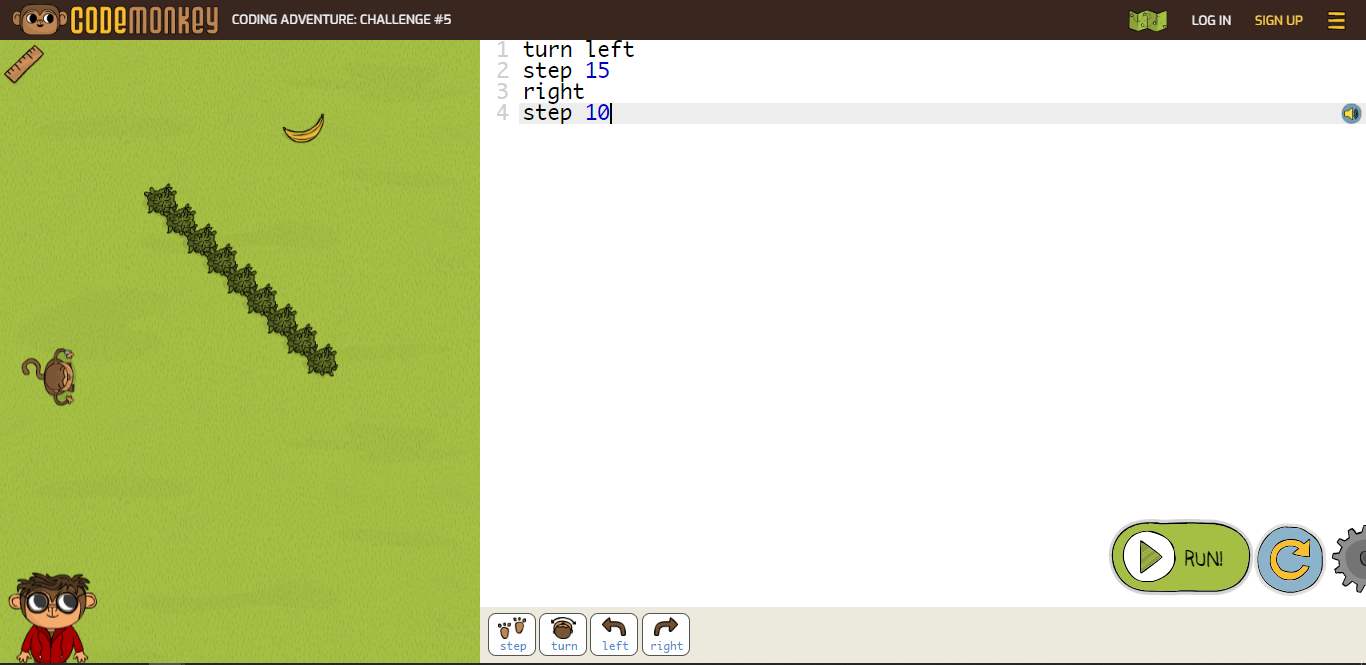
\includegraphics[width=15cm]{images/cap2/code_monkey.png}
    \caption*{Fonte:https://www.codemonkey.com/}
    \label{figura:code_monkey}
\end{figure}

Além de testes com ferramentas já conhecidas, podemos ver também na academia o desenvolvimento de novas soluções utilizando jogos digitais para trabalhar outros conceitos ou o próprio conceito da programação. No artigo \textit{"Towards a Tangible User Interface Embedded Computing Prototype For Child Education"} \cite{carneiro_2018}, foram desenvolvidos três jogos digitais com o objetivo de trabalhar e exercitar conceitos básicos de matemática para crianças que estão iniciando a alfabetização matemática. Além dos jogos, foi desenvolvido também uma base física que comportava seis blocos e os blocos numéricos individuais, ou seja, cada bloco com um número. Neste trabalho, os jogos propostos eram jogados por meio dessa estrutura física, como demonstrado na Figura \ref{figura:estrutura_artigo_towards}, para promover uma maior interação da criança com os jogos. Portanto, era proposto então um desafio matemático para a criança e após a resolução desse desafio, a criança deveria colocar na base os cubos numéricos com a resolução do desafio e apertar um botão para enviar sua resposta, para por fim receber uma mensagem de “correto” ou “incorreto”. Não houveram testes para comprovar a efetividade da solução. 

\begin{figure}[h!]
    \centering
    \caption{Estrutura Fisica do artigo \textit{"Towards a tangible user interface embedded computing prototype for child education”}}
    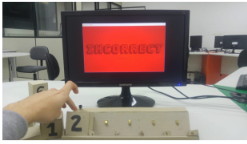
\includegraphics[width=10cm]{images/cap2/estrutura_artigo_towards.png}
    \caption*{Fonte: \cite{carneiro_2018}}
    \label{figura:estrutura_artigo_towards}
\end{figure}

Pode-se utilizar de jogos digitais para facilitar ou até mesmo possibilitar o ensino de disciplinas tradicionais na grade curricular brasileira, como por exemplo no artigo “Jogos Digitais No Ensino Da Língua Portuguesa Para Crianças Surdas” \cite{liz_2017} que utilizou jogos digitais para ensinar a língua portuguesa e em um contexto de acessibilidade. Neste artigo os pesquisadores relatam o projeto de Educomunicação feito pela Universidade Estadual de Campinas em parceria com uma escola municipal do estado de São Paulo. O objetivo foi desenvolver jogos digitais para tablets para possibilitar o ensino da língua portuguesa como língua secundária para alunos com deficiência auditiva de primeiro a quinto ano, em uma turma bilíngue. O método de validação, foi uma análise comparativa de desempenho baseado em duas atividades: uma das atividades continha palavras que foram trabalhadas nos jogos digitais e a segunda atividade continha palavras que não foram trabalhadas por meio desse recurso. Por meio da avaliação comparativa, pode-se ver que houveram mais respostas certas nas atividades com palavras que receberam intervenção dos jogos digitais desenvolvidos pelas pesquisadoras. Por fim, por meio dos testes, a  pesquisa pôde concluir que, jogos digitais são uma estratégia importante para o ensino da língua portuguesa para crianças com deficiência auditiva.

\subsection{Mercado}
Assim como no meio acadêmico, pode-se ver no mercado um movimento para o desenvolvimento de novas soluções digitais com foco na educação também. 
No ano de 2007, o \textit{Media Lab} do \textit{Massachusetts Institute of Technology} (MIT) desenvolveu uma linguagem de programação em blocos com o objetivo de ensinar crianças o pensamento criativo, trabalho colaborativo e pensamento sistemático, habilidades essenciais para o século XXI \cite{about_scratch}. Hoje, além de um ferramenta de programação, o Scratch é também uma comunidade online na qual crianças podem programar jogos, histórias e animações e compartilhar essas criações com o mundo, como pode-se ver na Figura \ref{figura:scratch}. O Scratch foi desenvolvido principalmente para crianças entre oito e dezesseis anos, mas segundo a própria ferramenta, é usado por milhões de pessoas de todas as idades. Hoje o scratch se encontra em casas e escolas de mais de cento e cinquenta países e é usado para trabalhar diversas disciplinas como matemática, ciência da computação, linguagens, artes, entre outras. Por conta de seu alcance, o Scratch está disponível em mais de quarenta línguas. Em 2016 a Scratch Foundation tornou pública uma parceria com a gigante Google para uma atualização da ferramenta, e o lançamento da versão 3.0 do Scratch ocorreu em janeiro de 2019.

\begin{figure}[h!]
    \centering
    \caption{Plataforma Scratch}
    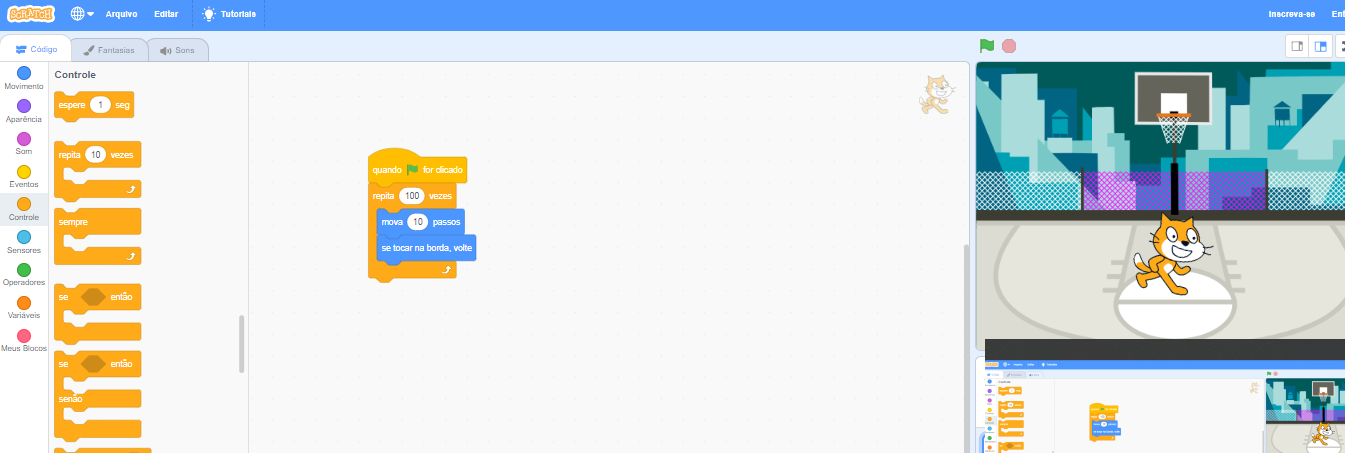
\includegraphics[width=15cm]{images/cap2/scratch.png}
    \caption*{Fonte: https://scratch.mit.edu/projects/editor/}
    \label{figura:scratch}
\end{figure}

Em 2015, a emissora britânica British Broadcasting Corporation (BBC), fez o anúncio da iniciativa Make it Digital com o objetivo de “inspirar os visionários digitais do futuro” como diz seu Diretor Geral Tony Hall. Parte dos esforços dessa iniciativa era o desenvolvimento de um microcomputador barato, portátil e fácil de programar, o que deu origem ao BBC micro:bit. O BBC micro:bit é uma placa de circuitos elétricos, tem um conector Universal Serial Bus (USB) para alimentação e transferência de dados, e, o que mais chama atenção na placa, é sua gama diversa de sensores como botões, termômetro, luxímetro, magnetrônomo e acelerômetro. Além disso, a placa conta com vinte e cinco leds vermelhos dispostos em uma matriz cinco por cinco e possui também contatos para conexão de periféricos externos. O objetivo da placa com todas essas possibilidades é, fazer com que as crianças tenham mais interesse por eletrônica e programação. Pensando na demanda das escolas de preparar profissionais com habilidades tecnológicas e, juntamente com as novas diretrizes da BNCC, a empresa brasileira Tecnologia Educacional com a solução Inventura, já colocou o BBC micro:bit em diversas escolas brasileiras em um material que, além de trabalhar competências técnicas, trabalha também competências como comunicação, colaboração, pensamento analítico, curiosidade, imaginação, entre outros \cite{about_microbit}. 

Segundo o World Economic Forum, sessenta e cinco por cento das crianças que estão entrando na escola primária hoje, terão trabalhos que ainda não existem. Pensando  nesses dados e observando toda essa mudança acontecendo no meio educacional, a empresa dinamarquesa de blocos de montar, LEGO, desenvolveu diversos produtos que permeiam esse contexto. Um dos mais famosos é o LEGO\textsuperscript{®} MINDSTORMS \textsuperscript{®} Education EV3, pensado para alunos do ensino médio e fundamental II. O Education EV3 é um produto de robótica educacional que incentiva o ensino STEAM (Science, Technology, Engineering, Art and Math). Além dos blocos de montar normais que são comuns nos produtos da empresa, o produto conta com o bloco EV3, que é um computador programável capaz de receber informação de sensores e controlar atuadores. O EV3 é programável através um software da mesma empresa disponível para tablets e computadores \cite{lego_mindstorms}. O software LabVIEW é um ambiente de programação gráfico que faz uso de blocos para estruturar comando para o EV3, como mostrado Figura \ref{figura:labview}, tornando a programação simples e intuitiva. 

\begin{figure}[h!]
    \centering
    \caption{Interface LabVIEW}
    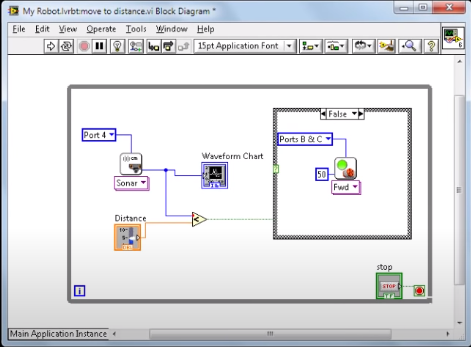
\includegraphics[width=10cm]{images/cap2/labview.png}
    \caption*{Fonte: \cite{labview}}
    \label{figura:labview}
\end{figure}

\subsection{Comentários}
Observa-se diversos esforços da academia e do mercado para desenvolver pesquisas, produtos e novas soluções para preparar as crianças que estão entrando agora no ensino básico para assumir futuros novos empregos. Esses esforços também focam em motivar e aprimorar o ensino dessas crianças por meio de novas estratégias educacionais, como  por exemplo jogos digitais. Pensando nisso, o trabalho proposto tem como objetivo ensinar programação por meio de jogos digitais como no artigo “Jogos Digitais no Ensino de Conceitos de Programação para Criança" \cite{tadesco_2016} que mostra as vantagens dessa metodologia para o ensino de programação para crianças. Fica claro por meio do artigo "Jogos Digitais No Ensino Da Língua Portuguesa Para Crianças Surdas" \cite{liz_2017} o potencial de jogos digitais para o ensino de diversas disciplinas, portanto este trabalho abordará o tema da reciclagem como cenário do jogo proposto com o objetivo de, além de programação, ensinar também sobre sustentabilidade. Considerando a importância de recursos que aumentam a interatividade das crianças com o ensino como visto no artigo \textit{"Towards a Tangible User Interface Embedded Computing Prototype For Child Education"} \cite{carneiro_2018}, o trabalho proposto, além do uso de jogos digitais, também fará uso de blocos físicos para promover uma maior interatividade com a criança tornando-a assim ainda mais protagonista do seu aprendizado. A escolha do uso dos blocos para o ensino da programação se deu por conta da comprovação de sua efetividade considerando a sua ampla utilização no mercado em soluções como o Scratch e do EV3 da Lego education, pois torna programação mais simples, interativa e intuitiva. 





\chapter{Especificação técnica} \label{cap:especificacao_tecnica}
Neste capítulo são apresentadas as especificações do sistema, as condições restritivas, benefícios e impactos, análise funcional e de requisitos, a arquitetura do sistema e seus custos.

\section{Análise de Contexto}

    O desenvolvimento deste protótipo tem a finalidade de auxiliar o professor no ensino de programação para crianças.
    
    \subsection{Visão Geral}
    
    O software, em forma de jogo com o tema reciclagem, apresentará diversos desafios em que a criança deverá solucionar criando sequências lógicas com blocos físicos, conforme apresentado na Figura \ref{figura:visao_geral}. O objetivo do jogo é levar o personagem principal para coletar o lixo, descartado incorretamente no chão, e descartá-lo na lixeira correta. Para movimentar o personagem no cenário, a criança ordenará blocos físicos em uma superfície plana. Cada bloco possui cor e símbolo próprio para representar a sua ação. Após a ordenação dos blocos, de maneira em que a criança achar correta, ela deverá tirar uma foto da sua solução e submetê-la para a análise do servidor conforme apresentado no diagrama da Figura \ref{figura:blocos_desafio}.
    
    \begin{figure}[H]
        \caption{Visão geral do sistema}
        \centering
        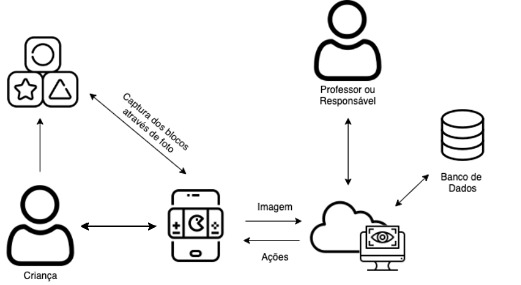
\includegraphics[width=\linewidth]{Imagens/Cap3/Visao_Geral.jpg}
        \legend{\small{Fonte: o autor (2020)}}
        \label{figura:visao_geral}
    \end{figure}
    
    \begin{figure}[H]
        \caption{Diagrama de blocos para submissão do desafio}
        \centering
        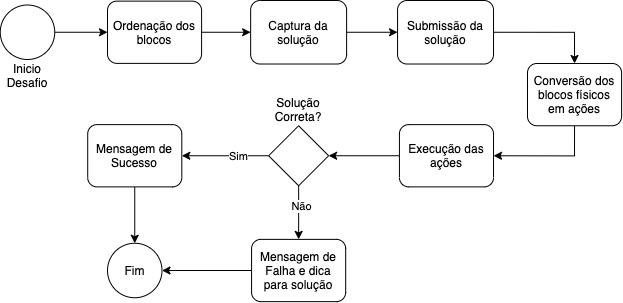
\includegraphics[width=\linewidth]{Imagens/Cap3/Blocos Desafio.jpg}
        \legend{\small{Fonte: o autor (2020)}}
        \label{figura:blocos_desafio}
    \end{figure}
    
    A análise da imagem será por meio de visão computacional a fim de identificar os blocos utilizados e convertê-los em ações. Ao final da conversão, o servidor salvará a solução submetida no banco de dados e retornará as ações para o jogo executar, representado no diagrama da Figura \ref{figura:blocos_reconhecimento}. O professor/tutor terá acesso a um link para visualizar todas as submissões das crianças, além de gráficos estatísticos comparando os resultados das crianças.
    
    \begin{figure}[H]
        \caption{Diagrama de blocos para reconhecimento dos blocos}
        \centering
        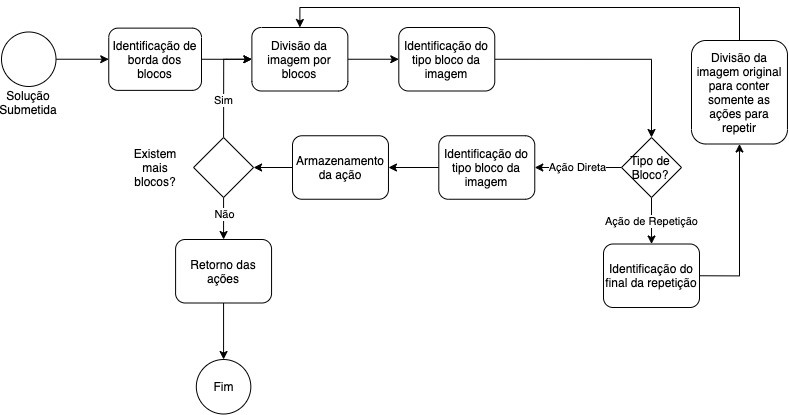
\includegraphics[width=\linewidth]{Imagens/Cap3/Blocos Reconhecimento.jpg}
        \legend{\small{Fonte: o autor (2020)}}
        \label{figura:blocos_reconhecimento}
    \end{figure}
    
    \subsection{Condições Restritivas}
    O projeto proposto apresenta algumas condições restritivas, conforme descrito nos próximos subitens.

        \subsubsection{Custos}
        Apesar do jogo precisar de materiais relativamente baratos para ser jogado, como blocos impressos em 3D e também se faz necessário o uso de um celular com sistema operacional Android com câmera para que o aplicativo funcione. 
        
        São necessários 20 blocos para jogar o jogo de forma completa, ou seja, todas as fases. O preço médio de 1kg de filamento de PLA na data da escrita deste documento, considerando diferentes cores e frete, o que é necessário para distinção dos blocos, é de R\$150,00. Portanto, considerando que cada blocos possui 10cm x 10cm x 5mm, estima-se o custo de R\$10,00 por bloco, totalizando um total de R\$200,00.
            
        \subsubsection{Físicas e Ambientais}
        Apesar, quando impressos em 3D, dos blocos terem uma boa durabilidade, com o passar do tempo ficarão inutilizáveis. Portanto deve-se orientar os usuários do jogo a fazer o descarte adequado dos blocos físicos depois de se tornarem inutilizáveis, seja por desgaste dos blocos ou por falta de uso, o que vai ao encontro com uma das propostas levantada pelo aplicativo jogo, a reciclagem.
        
        \subsubsection{Tecnológicas}
        O aplicativo jogo necessita de um celular com câmera e com o sistema operacional Android com a versão igual ou superior a 5.0 - Lollipop. Por se tratar de um protótipo, o aplicativo não oferece suporte para os demais dispositivos móveis com outros sistemas operacionais, como por exemplo iPhone. 
        
        \subsubsection{Energização}
        O dispositivo móvel é limitado em relação à energia, tendo um período máximo que uma carga pode sustentar, esse período máximo varia conforme o modelo e o uso do dispositivo. Para diminuir os efeitos causado por essa limitação, recomenda-se o uso do aplicativo com a bateria cheia ou próximo a uma tomada caso seja necessário recarregar a bateria do dispositivo móvel.    
        
        \subsubsection{Interferências devido ao meio}
        O aplicativo jogo precisa de conexão com internet para funcionar. Obstáculos como objetos metálicos ou paredes podem causar interferências no sinal Wi-Fi. Eletrônicos e eletrodomésticos, como por exemplo micro-ondas, operam na mesma frequência do roteador wireless, 2,4 GHz, que quando ligados, também podem contribuir com interferências dificultando ou até impossibilitando o uso do aplicativo.
        
        O captura das imagens no jogo também precisará ser feita sob luz ambiente, não escuro e também não sob incidência solar. A captura das imagens também deverá ser realizada segundo as orientações de posicionamento que o jogo dará. O não cumprimento dessas orientações pode impactar diretamente no funcionameto do jogo.
    
    \subsection{Benefícios e Impactos}
    O aplicativo jogo apresenta alguns benefícios e impactos, conforme descrito nos próximos subitens.

        \subsubsection{Econômicos}
        Além de um celular com câmera, o aplicativo jogo proposto é capaz de funcionar com recursos relativamente baratos, como blocos impressos em 3D; jogo também funciona de forma simples. Portanto pode ser utilizado em casa ou implantado em escolas de forma fácil e econômica para proporcionar às crianças um contato inicial com temas como lógica de programação e sustentabilidade, além de atender às novas demandas da BNCC para o ensino.
        
        \subsubsection{Operacionais}
        O jogo pode ser aplicado em ambiente escolar. Por ser uma ferramenta que difere dos métodos tradicionais de ensino das escolas, pode ser uma experiência lúdica o que impacta diretamente na rotina das crianças. Porém para utilização em ambiente escolar, recomenda-se uma sala com um amplo espaço para posicionamento dos blocos e um profissional da educação para monitorar o uso.
        
        \subsubsection{Estratégicos}
        A mais nova atualização da Base Nacional Comum Curricular destina uma de suas dez competência à educação integral por meio de tecnologias digitais e faz uso, no caderno de matemática, do termo “pensamento computacional”. Pensando nisso, o aplicativo jogo proposto possibilita, de uma forma estratégica, um meio para trabalhar essas competências nas escolas. 
        
        \subsubsection{Políticos}
        Não se aplica.

        \subsubsection{Sociais}
        O aplicativo jogo apresenta benefícios sociais para as crianças, pois as crianças terão acessos a conceitos básicos de lógica de programação e oportunidade de exercitar esse conceito, o que pode auxiliar em competências como raciocínio lógico, resolução de problemas, pensamento computacional, entre outras habilidades que tem sido cada vez mais requisitadas no mercado de trabalho. Sendo esses conceitos trabalhados por meio de um jogo, além de gerar maior engajamento por parte das crianças, pode desenvolver também, competências como cooperação, cumprimento de regras, controle de impulsividade, auxílio na tomada de decisões, mais facilidade para lidar com erros e fracassos entre outras habilidades sociais que jogos são capazes de desenvolver.
        Além disso, o jogo, por meio do tema de reciclagem, pode desenvolver senso de sustentabilidade auxiliando na compreensão da importância do descarte correto do lixo, o que impacta direta e positivamente  o meio ambiente.
        % Revisar escrita

\section{Análise Funcional e de Requisitos Tecnológicos}
    Nessa sessão, é apresentada a análise funcional e os requisitos tecnológicos do sistema.

    \subsection{Lista de Funcionalidade e Atores}
    O sistema será composto  pelas seguintes funcionalidades:
    \begin{itemize}
        \item Desafios de lógica com o tema reciclagem;
        \item Identificação dos blocos;
        \item Conversão dos blocos em ações;
        \item Relatórios de jogo para acompanhamento do professor.
    \end{itemize}
    
    O sistema tem como atores a criança e o professor/tutor. A criança é responsável pela interação com os blocos e aplicativo.
    O professor/tutor é responsável pela interação com os dados adquiridos durante a partida jogada pela criança.
    
    \subsection{Comunicação}
    A comunicação entre o aplicativo e o servidor ocorrerá de maneira bidirecional e utilizará arquitetura \textit{REST}, através da conexão Wi-Fi com a Internet.
    O aplicativo envia os dados e imagens para o servidor. Após o servidor salvar os dados e processar as imagens, ele retorna as ações para serem executadas no aplicativo.
    
    O \textit{REST (Representational State Transfer)} é uma abstração da arquitetura da \textit{Web}. Consistem em regras que permitem a criação de projetos com interfaces bem definidas, permitindo a comunicação entre aplicações.
    
    \subsection{Processamento}
    
      O processamento por parte do software, ocorre tanto no aplicativo quanto no servidor. O jogo captura as imagens e as envia para o servidor através da Internet. O servidor recebe as imagens enviadas pelo aplicativo e passa cada uma pelo algoritmo de visão computacional, responsável pela identificação de cada bloco nas fotos. Após a identificação dos blocos, é salvo a sequência no banco de dados e as ações são enviadas para o aplicativo.
    
     Após receber o retorno com as ações, o aplicativo transforma as ações em código e executa o mesmo durante o jogo.
     
    \subsubsection{Jogo}
  
    O jogo possuirá 4 desafios, cada um explorando um tipo de bloco. Ao inicio de cada fase, será executado uma animação para mostrar a ação que o tipo de bloco apresentado na fase executará juntamente com a sua forma de utilização.
    
    A primeira fase, apresentada na Figura \ref{figura:fase_1} trabalha a utilização do bloco "andar". Para completar a fase com sucesso, a criança precisará utilizar uma combinação de três blocos andar para coletar o lixo e levá-lo a lixeira correta. Ao final dessa fase, será apresentado um vídeo informativo sobre o descarte correto de plástico.
    
    \begin{figure}[H]
        \caption{Fase 1}
        \centering
        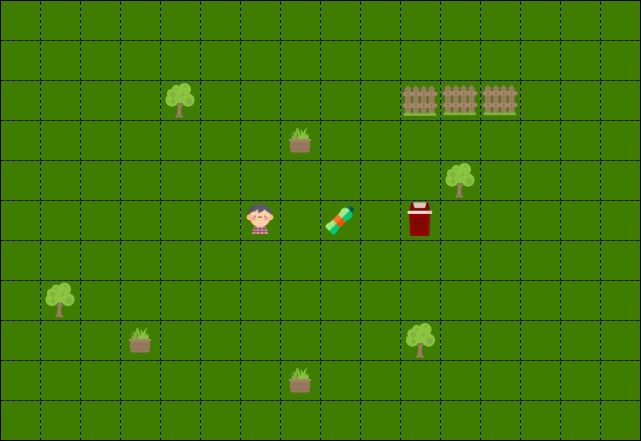
\includegraphics[width=12cm]{Imagens/Cap3/Fases/Fase1.jpg}
        \legend{\small{Fonte: o autor (2020)}}
        \label{figura:fase_1}
    \end{figure}
    
    A segunda fase, apresentada na Figura \ref{figura:fase_2} trabalha a utilização do bloco "virar a noventa graus". Para completar a fase com sucesso, a criança precisará utilizar uma combinação de quatro blocos andar e um bloco virar 90 graus para coletar o lixo e levá-lo a lixeira correta. Ao final dessa fase, será apresentado um vídeo de instrução sobre o descarte correto de papel.
    
    \begin{figure}[H]
        \caption{Fase 2}
        \centering
        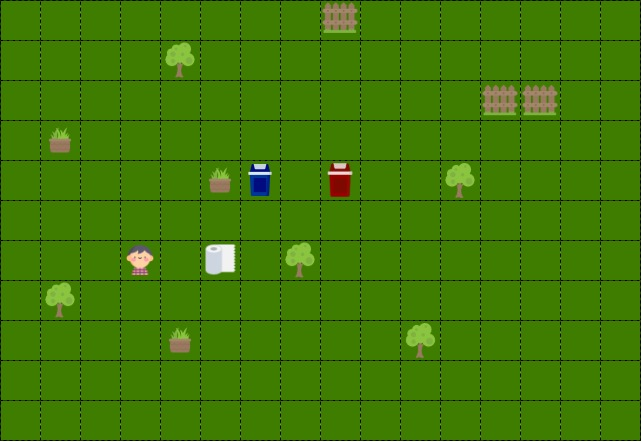
\includegraphics[width=12cm]{Imagens/Cap3/Fases/Fase2.jpg}
        \legend{\small{Fonte: o autor (2020)}}
        \label{figura:fase_2}
    \end{figure}
    
    A terceira fase, apresentada na Figura \ref{figura:fase_3} trabalha a utilização do bloco "esperar". Para completar a fase com sucesso, a criança precisará utilizar uma combinação de cinco blocos andar e um bloco esperar para coletar o lixo e levá-lo a lixeira correta. Ao final dessa fase, será apresentado um vídeo informativo sobre o descarte correto de metal.
    
    \begin{figure}[H]
        \caption{Fase 3}
        \centering
        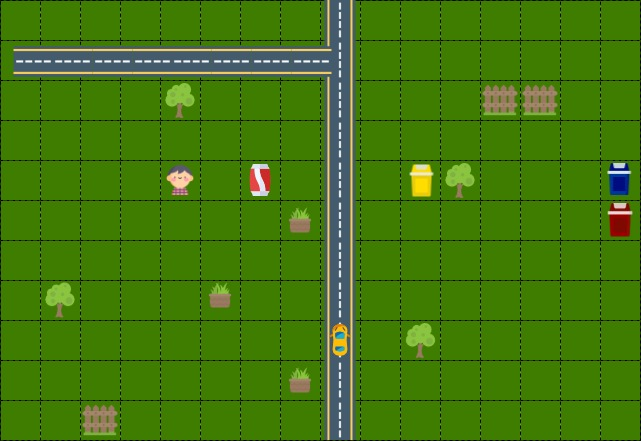
\includegraphics[width=12cm]{Imagens/Cap3/Fases/Fase3.jpg}
        \legend{\small{Fonte: o autor (2020)}}
        \label{figura:fase_3}
    \end{figure}
    
    A quarta fase, apresentada na Figura \ref{figura:fase_4} trabalha a utilização do bloco de "repetição". Para completar a fase com sucesso, a criança precisará utilizar uma combinação de quatro blocos andar, um bloco esperar e um bloco virar 90 graus juntamente do bloco de repetição e o bloco numérico 2 para coletar o lixo e levá-lo a lixeira correta. Ao final dessa fase, será apresentado um vídeo informativo sobre o descarte correto de vidro.
    
    \begin{figure}[H]
        \caption{Fase 4}
        \centering
        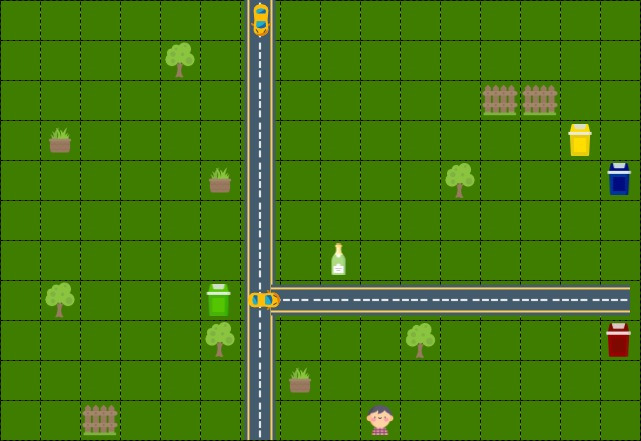
\includegraphics[width=12cm]{Imagens/Cap3/Fases/Fase4.jpg}
        \legend{\small{Fonte: o autor (2020)}}
        \label{figura:fase_4}
    \end{figure}


    \subsubsection{Reconhecimento dos blocos}
     
     Para etapa de reconhecimentos dos blocos será utilizado a linguagem de programação Python versão 3 juntamente com o módulo de processamento digital de imagens OpenCV.

    
    
    \subsection{Interface Homem-Máquina}
    As interações da criança serão com os blocos físicos e com o aplicativo.
    Na tela inicial, são apresentadas duas opções, créditos e desafios, como mostra a Figura \ref{figura:tela_inicial}.
    
    \begin{figure}[H]
        \caption{Tela Inicial}
        \centering
        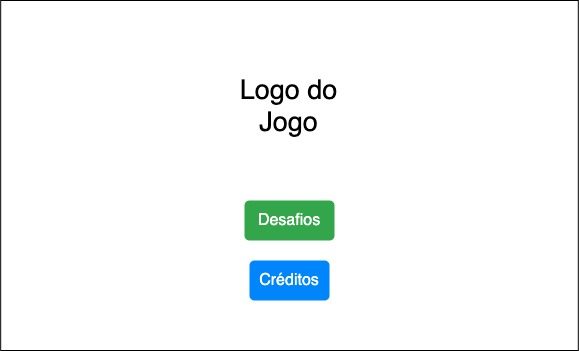
\includegraphics[width=\linewidth]{Imagens/Cap3/Tela Inicial.jpg}
        \legend{\small{Fonte: o autor (2020)}}
        \label{figura:tela_inicial}
    \end{figure}
    
    Ao acessar a opção de desafios é apresentada a lista de todos os desafios disponíveis, juntamente com o progresso de cada desafio (se disponível), conforme apresentado na Figura \ref{figura:tela_desafios}.
    
    \begin{figure}[H]
        \caption{Tela de Desafios}
        \centering
        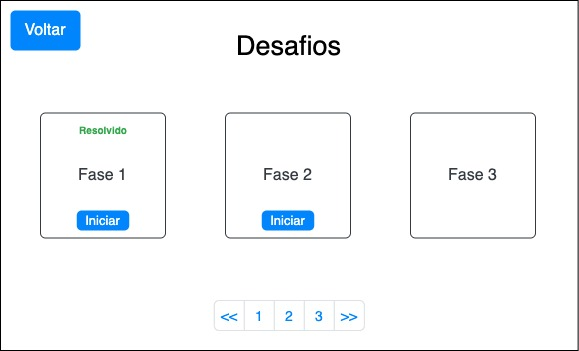
\includegraphics[width=\linewidth]{Imagens/Cap3/tela_desafios.jpg}
        \legend{\small{Fonte: o autor (2020)}}
        \label{figura:tela_desafios}
    \end{figure}
    
    Nessa tela, é possível ver a lista de desafios, um desafio só poderá ser iniciado caso o anterior tenha sido resolvido.
    É possível clicar no botão "voltar" para retornar à tela anterior. Ao clicar no botão "iniciar" do desafio, a criança poderá ser direcionada para a tela de cadastro ou direto para a tela do desafio. Caso a criança não tenha preenchido as informações para identificá-la, essas informações serão coletadas em uma tela específica, conforme Figura \ref{figura:cadastro}. Caso contrário ela é direcionada para a tela que contém o desafio a ser solucionado.
    
    \begin{figure}[H]
        \caption{Tela de Cadastro}
        \centering
        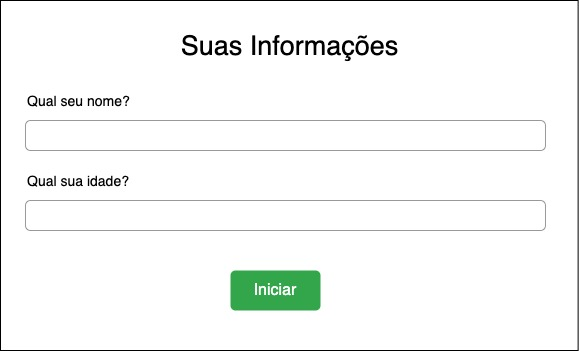
\includegraphics[width=\linewidth]{Imagens/Cap3/informacoes_usuario.jpg}
        \legend{\small{Fonte: o autor (2020)}}
        \label{figura:cadastro}
    \end{figure}
    
    A Figura \ref{figura:tela_jogo} mostra a interface principal durante o jogo.
    
    \begin{figure}[H]
        \caption{Tela do Jogo}
        \centering
        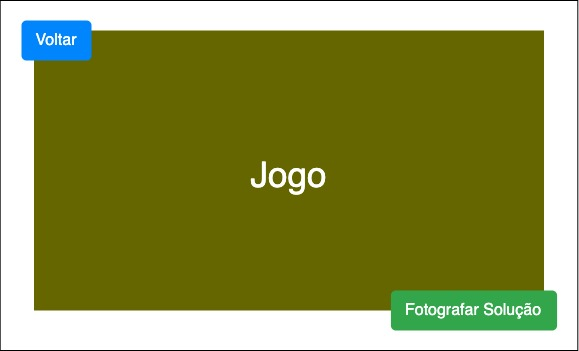
\includegraphics[width=\linewidth]{Imagens/Cap3/tela_jogo.jpg}
        \legend{\small{Fonte: o autor (2020)}}
        \label{figura:tela_jogo}
    \end{figure}
    
    Nessa tela é possível executar duas ações. Clicando no botão "voltar", a criança é redirecionada para a lista de desafios. Selecionando o botão "Fotografar Solução", é aberta uma janela, conforme Figura \ref{figura:fotografar_blocos} para fotografar a solução.
    
    \begin{figure}[H]
        \caption{Tela para fotografar a solução}
        \centering
        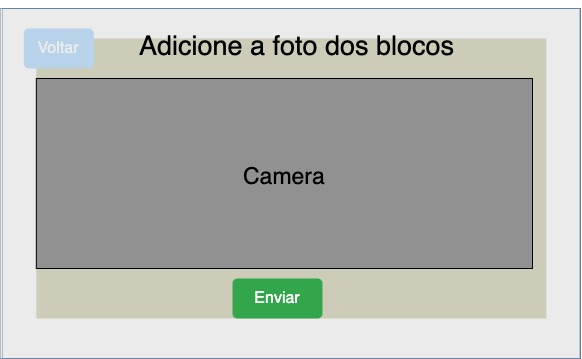
\includegraphics[width=\linewidth]{Imagens/Cap3/UploadSolucao.jpg}
        \legend{\small{Fonte: o autor (2020)}}
        \label{figura:fotografar_blocos}
    \end{figure}
    
    Cada bloco deve ser fotografado e adicionado utilizando o botão "Novo Bloco".
    Ao fotografar todos os blocos, pode-se clicar no botão enviar para que a solução seja processada.
    Após a conversão da foto em ações para o jogo, o usuário é direcionado para a tela de jogo onde as ações convertidas serão executadas.
    Caso o personagem chegue com o lixo na lixeira correta , será apresentada uma mensagem de sucesso, conforme Figura \ref{figura:solucao_correta}. Caso contrário, será apresentada a mensagem de falha, permitindo uma nova tentativa, Figura \ref{figura:solucao_incorreta}.
    
    \begin{figure}[H]
        \caption{Mensagem de solução correta}
        \centering
        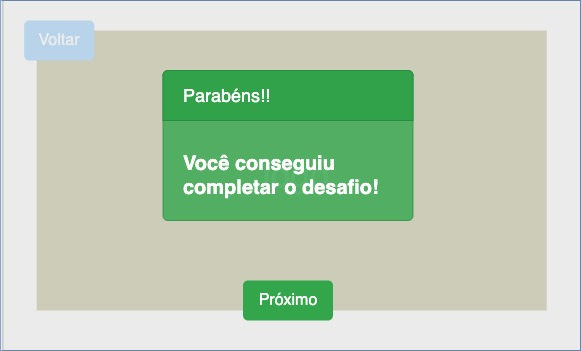
\includegraphics[width=\linewidth]{Imagens/Cap3/solucao_correta.jpg}
        \legend{\small{Fonte: o autor (2020)}}
        \label{figura:solucao_correta}
    \end{figure}
    
    \begin{figure}[H]
        \caption{Mensagem de solução incorreta}
        \centering
        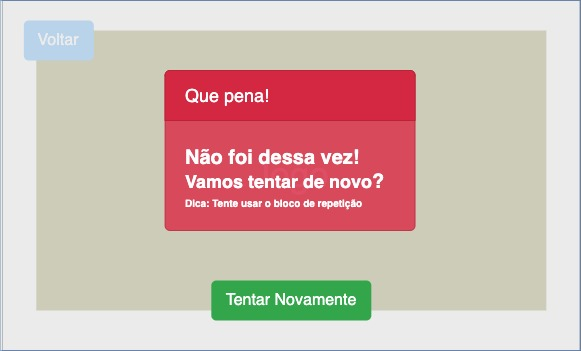
\includegraphics[width=\linewidth]{Imagens/Cap3/solucao_incorreta.jpg}
        \legend{\small{Fonte: o autor (2020)}}
        \label{figura:solucao_incorreta}
    \end{figure}
    
    O tutor terá acesso a um link para visualizar o relatório com as submissões das crianças conforme mostra a Figura \ref{figura:tela_relatorios}. Será possível ver todas as soluções enviadas além de relatórios estatísticos sobre o progresso no jogo.
    
    \begin{figure}[H]
        \caption{Tela de Relatórios}
        \centering
        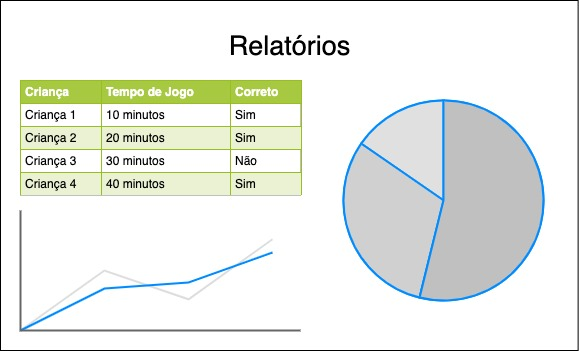
\includegraphics[width=\linewidth]{Imagens/Cap3/Tela Relatorios.jpg}
        \legend{\small{Fonte: o autor (2020)}}
        \label{figura:tela_relatorios}
    \end{figure}
    
    \subsection{Sistemas Controlados Automaticamente}
    O Sistema não apresentará sistemas controlados automaticamente.
    
    \subsection{Aquisição de dados e Atuação}
    A coleta das fotos se dará por meio da ação da criança que está jogando. Após concluir a proposta de solução do desafio, a criança deve capturar sua proposta utilizando a câmera do dispositivo móvel, como mostrado na Figura \ref{figura:crianca_blocos}.
    
    \begin{figure}[H]
        \caption{Criança capturando a solução}
        \centering
        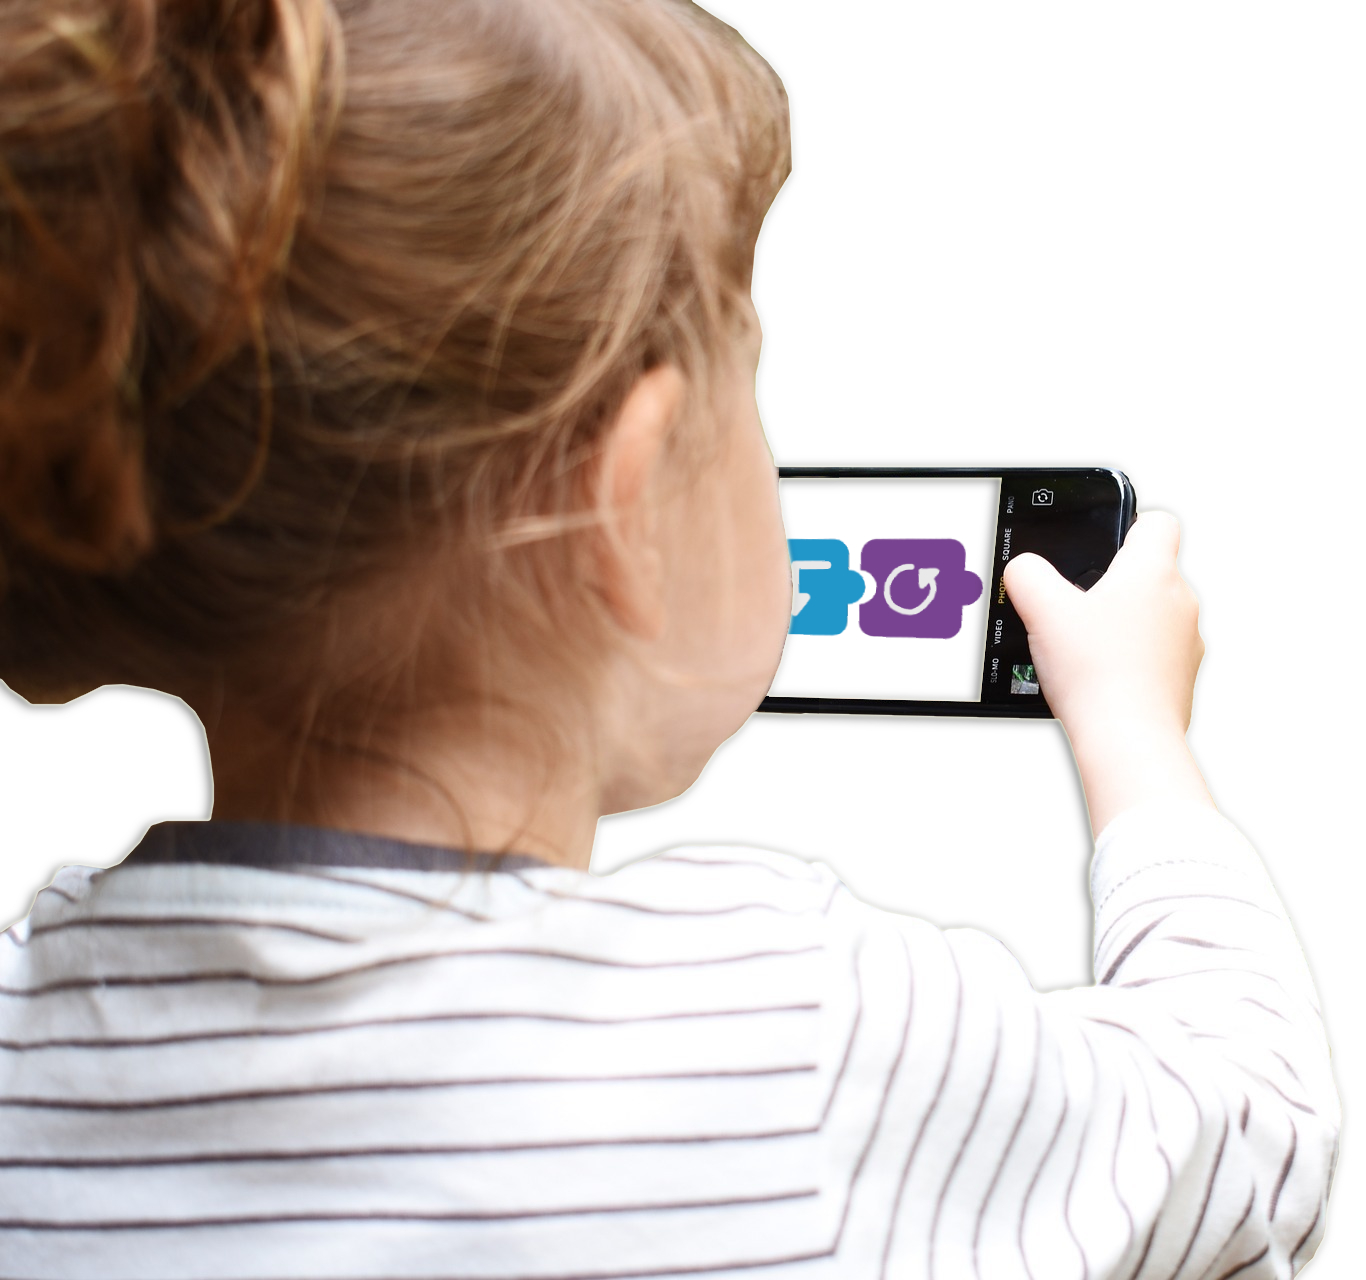
\includegraphics[width=10cm]{Imagens/Cap3/CriançaBlocos.jpg}
        \legend{\small{Fonte: o autor (2020)}}
        \label{figura:crianca_blocos}
    \end{figure}
    
    Após a captura da imagem, a criança, utilizando um botão de envio, submeterá a foto para o servidor.
    
    O envio da foto e o recebimento da conversão em ações do jogo é realizado através de conexão com a Internet.
    Toda proposta de solução, esteja ela correta ou não, será salva no banco de dados, após sua interpretação, para gerar relatórios estatísticos.


\section{Análise da Arquitetura do Sistema}
    Nessa sessão, são apresentadas as arquiteturas de hardware e software do sistema.

    \subsection{Hardware}
    O hardware do sistema será composto por blocos físicos e o dispositivo mobile com câmera. O dispositivo mobile deverá ser um celular \textit{Android} com câmera, podendo variar entre os modelos existentes no mercado.
    
    Os blocos físicos serão construídos de PLA, impressos em 3D, com o tamanho aproximado de 10cm x 10cm x 5mm, seus cantos serão arredondados para evitar acidentes no manuseio. Para facilitar a identificação, cada bloco possuirá uma cor especifica juntamente com um símbolo representando a sua ação.
    Os blocos são dividos em duas categorias, sendo elas, ações e blocos numéricos. As ações são divididas em dois tipos, ações diretas e repetição. A Figura \ref{figura:blocos_fisicos} apresenta todos os blocos disponíveis no protótipo.
    
    \begin{figure}[H]
        \caption{Blocos Físicos}
        \centering
        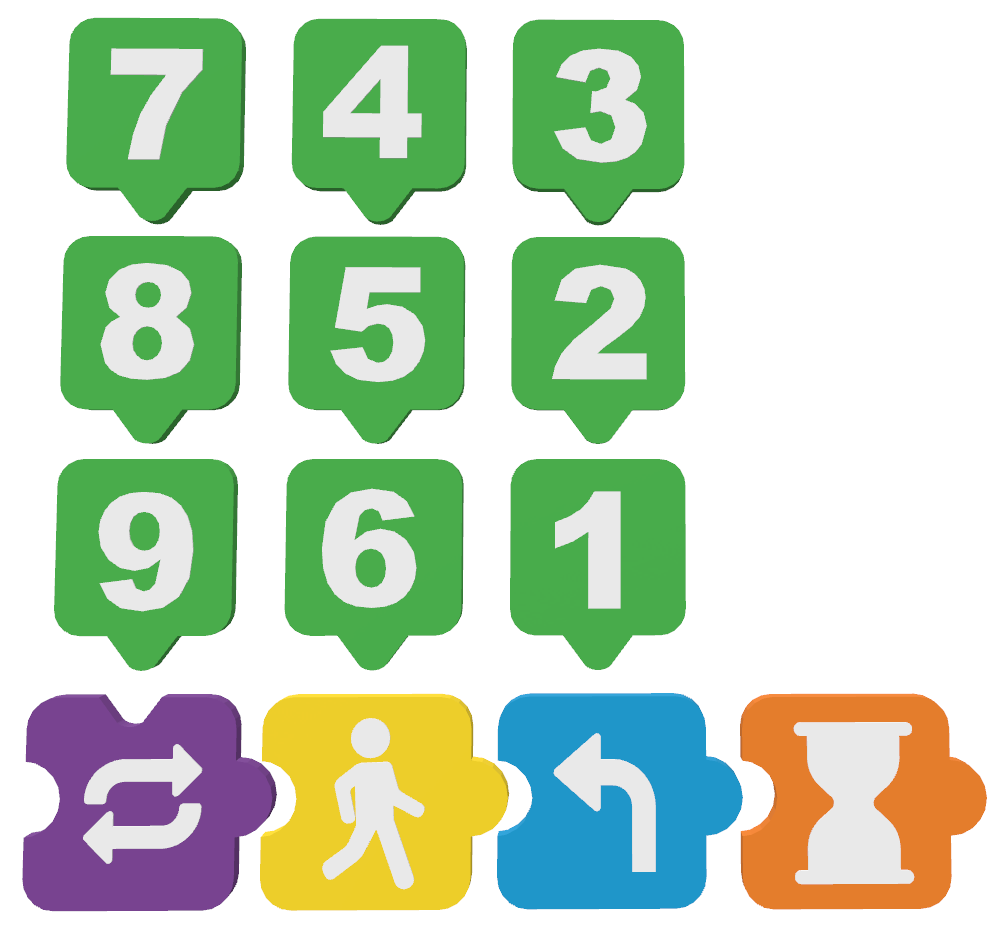
\includegraphics[width=\linewidth]{Imagens/Cap3/Blocos/Todos.png}
        \legend{\small{Fonte: o autor (2020)}}
        \label{figura:blocos_fisicos}
    \end{figure}
    
    \subsubsection{Blocos Numéricos}
        Os blocos numéricos são identificados pela cor verde e pelos números de um a nove, conforme apresentado na Figura \ref{figura:blocos_numericos}. Eles possuem um encaixe diferente dos demais e por isso somente encaixam nos blocos de repetição, pois são utilizados para identificar a quantidade de vezes que o bloco de repetição irá repetir. Tais blocos númericos não podem ser utilizados com outros blocos ou até mesmo sozinhos.
        
        \begin{figure}[H]
            \caption{Blocos Numéricos}
            \centering
            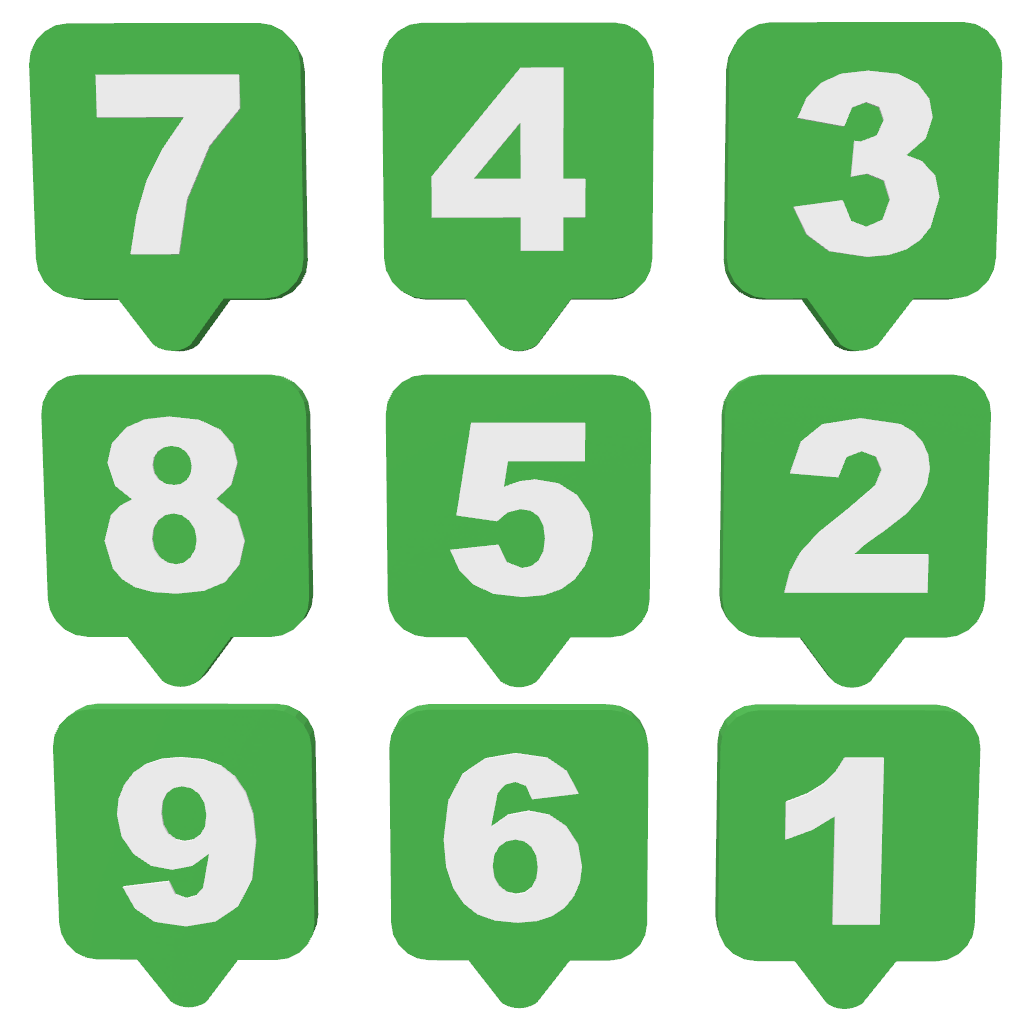
\includegraphics[width=10cm]{Imagens/Cap3/Blocos/Blocos_Numericos.png}
            \legend{\small{Fonte: o autor (2020)}}
            \label{figura:blocos_numericos}
        \end{figure}
    
    \subsubsection{Ações Diretas}
        As ações diretas são ações que não possuem necessidade de outros blocos, ou seja, podem ser utilizadas sozinhas.
        O jogo possui 3 ações diretas, sendo elas, "andar", "virar noventa graus" e "esperar". 
        A ação "andar" movimenta o personagem para frente uma única vez, seu bloco é identificado pela cor amarela e pelo simbolo de um boneco andando, conforme apresentado na Figura \ref{figura:andar}.
        
        \begin{figure}[H]
            \caption{Andar}
            \centering
            
\includegraphics[width=5cm]{Imagens/Cap3/Blocos/Andar.png}
            \legend{\small{Fonte: o autor (2020)}}
            \label{figura:andar}
        \end{figure}
        
        A ação "virar noventa graus" rotaciona o personagem noventa graus para a esquerda, seu bloco é identificado pela cor azul e o simbolo de uma seta apontando para a esquerda, conforme apresentado na Figura \ref{figura:virar}.
        
        \begin{figure}[H]
            \caption{Virar noventa graus}
            \centering
            
\includegraphics[width=5cm]{Imagens/Cap3/Blocos/Virar.png}
            \legend{\small{Fonte: o autor (2020)}}
            \label{figura:virar}
        \end{figure}
        
        A ação "esperar"' mantém o personagem parado no cenário, sem executar nenhuma outra ação, seu bloco é identificado pela cor laranja e o simbolo de uma ampulheta, conforme apresentado na Figura \ref{figura:esperar}
        
        \begin{figure}[H]
            \caption{Esperar}
            \centering
            
\includegraphics[width=5cm]{Imagens/Cap3/Blocos/Esperar.png}
            \legend{\small{Fonte: o autor (2020)}}
            \label{figura:esperar}
        \end{figure}
        
    \subsubsection{Ação de Repetição}
        A "ação de repetição" é identificada pela cor roxa e pelo símbolo de duas flechas em formato oval, conforme apresentado na Figura \ref{figura:repetir}. É uma ação que possui necessidade de mais blocos para ser executada, não podendo ser utilizada sozinha.
        
        \begin{figure}[H]
            \caption{Repetir}
            \centering
            
\includegraphics[width=5cm]{Imagens/Cap3/Blocos/Repetir.png}
            \legend{\small{Fonte: o autor (2020)}}
            \label{figura:repetir}
        \end{figure}
        
        Para criar uma repetição é preciso a utilização de um bloco de repetição seguido das ações diretas a serem repetidas e outro bloco de "repetição" para "finalização". Possui um encaixe na parte superior para ser colocado um bloco numérico, que identificará a quantidade de vezes que as ações devem ser executadas. O bloco numérico precisará constar somente no bloco de repetição de inicio. Caso não seja utilizado um bloco numérico em conjunto, ficará executando infinitamente. A Figura \ref{figura:exemplo_repeticao} mostra um exemplo de repetição, onde as ações "andar" e "virar noventa graus" serão repetidas infinitamente.
        
        \begin{figure}[H]
            \caption{Exemplo de repetição}
            \centering
            
\includegraphics[width=\linewidth]{Imagens/Cap3/Blocos/Exemplo_Repeticao.png}
            \legend{\small{Fonte: o autor (2020)}}
            \label{figura:exemplo_repeticao}
        \end{figure}
    
    \subsection{Software}
    O jogo será desenvolvido para celulares Android utilizando o Unity 3D. A arquitetura do software para reconhecimento dos blocos será baseada em serviços cloud, utilizando a IBM Cloud como provedor.
    O servidor, programado em Python, utilizará o serviço IBM Cloud Foundry. O banco de dados, não relacional, utilizará o serviço IBM Cloudant.
    
    O \emph{Cloud Foundry} é um servico \textit{PAAS (Platform as a Service)} que permite implementar e ajustar a escala de aplicativos de maneira rápida, simples e barata. O IBM Cloudant é um serviço de banco de dados distribuído, desenvolvido no Apache CouchDB, que é otimizado para grandes cargas e rápido crescimento.
    
    Nos tópicos a seguir, são apresentados os diagramas do software que representam o seu funcionamento.
        
        \subsubsection{Use Case}
        O jogo conta com funções de identificação da criança (perfil), inicio de desafio e submissão de solução, conforme apresentado no diagrama de caso de uso da criança na Figura \ref{figura:use_case}. A função de submissão de solução do jogo conversa diretamente com a função de reconhecimento dos blocos no servidor.
        O servidor conta com funções de relatórios e reconhecimento dos blocos. Apenas o professor/tutor poderá acessar os relatórios conforme apresentado no diagrama de caso de uso do tutor na Figura \ref{figura:use_case}.
        
        \begin{figure}[H]
            \caption{Caso de uso}
            \centering
                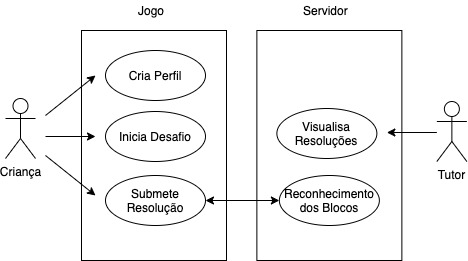
\includegraphics[width=15cm]{Imagens/Cap3/Use_Case.jpg}
            \legend{\small{Fonte: o autor (2020)}}
            \label{figura:use_case}
        \end{figure}
        
        \subsubsection{Diagramas de Sequência}
        
        Nesse tópico são apresentados os diagramas de sequência para as funcionalidades principais do aplicativo.
        
        \subsubsubsection{Criação de Perfil}
        
        A Figura \ref{figura:sequencia_perfil} mostra o diagrama de sequência para a realização do cadastro de informações da criança. Todas as informações são salvas localmente para que, na submissão da solução, seja salvo um único objeto. 
        
        \begin{figure}[H]
            \caption{Diagrama de Sequência - Perfil}
            \centering
                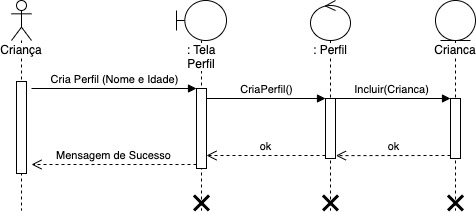
\includegraphics[width=\linewidth]{Imagens/Cap3/Sequencia_Perfil.jpg}
    
            \legend{\small{Fonte: o autor (2020)}}
            \label{figura:sequencia_perfil}
        \end{figure}
        
        \subsubsubsection{Submissão da Resolução}
        
        O diagrama apresentado na Figura \ref{figura:sequencia_jogo} mostra o processo de submissão da solução e validação da mesma.
        
        \begin{figure}[H]
            \caption{Diagrama de Sequência - Submissão da Resolução}
            \centering
                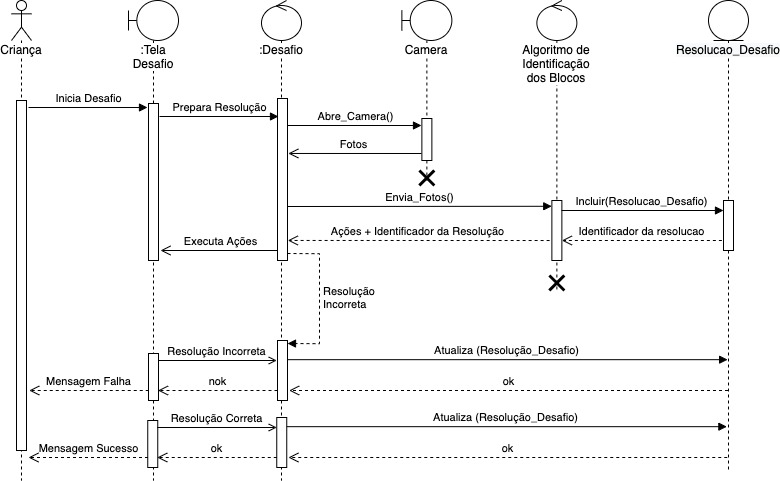
\includegraphics[width=\linewidth]{Imagens/Cap3/Sequencia_Jogo.jpg}
    
            \legend{\small{Fonte: o autor (2020)}}
            \label{figura:sequencia_jogo}
        \end{figure}
        
        Ao iniciar o desafio, a data e hora são salvos localmente para que, quando a resolução for submetida, essa informação seja salva junto com as demais no banco de dados. Após o aplicativo processar as ações convertidas pelo algoritmo de identificação dos blocos, o aplicativo valida a solução e atualiza a resolução no banco com o seu status, correto ou não correto.
        
        \subsubsubsection{Visualização de Relatório}
        
        O diagrama apresentado na Figura \ref{figura:sequencia_tutor} mostra o processo para o tutor visualizar os relatórios dos desafios submetidos pelas crianças.
        
        \begin{figure}[H]
            \caption{Diagrama de Sequência - Visualização de Relatório}
            \centering
                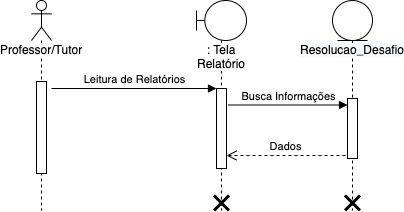
\includegraphics[width=\linewidth]{Imagens/Cap3/sequencia_tutor.jpg}
            \legend{\small{Fonte: o autor (2020)}}
            \label{figura:sequencia_tutor}
        \end{figure}
        
        O tutor receberá um link via e-mail para acessar o relatório das soluções submetidas pelas crianças. Ao acessar o link, a tela acessa o banco de dados para buscar as informações para popular os relatórios.
\clearpage

\addcontentsline{toc}{chapter}{REFÊRENCIAS}
\bibliography{bibli}

% \newpage

\end{document}